%%%%%%%%%%%%%%%%%%%%%%%%%%%%%%%%%%%%%%%%%%%%%%%%%%%%%%%%%%%%%%%%%%%%%%%%%%%%%%%%%%
\begin{frame}[fragile]\frametitle{}
\begin{center}
{\Large ReAct Agent from Scratch with a Small Local Model}

{\tiny (Ref: ReAct agent from scratch with Gemini and LangGraph - Gemini API docs; here run on a small model through LM Studio)}
\end{center}
\end{frame}

%%%%%%%%%%%%%%%%%%%%%%%%%%%%%%%%%%%%%%%%%%%%%%%%%%%%%%%%%%%
\begin{frame}[fragile]\frametitle{What is a ReAct Agent?}
      \begin{itemize}
        \item \textbf{ReAct} = Reasoning + Acting (Yao et al., 2022, arXiv 2210.03629).
        \item \textbf{Loop}: Think \(\rightarrow\) Act (tool call) \(\rightarrow\) Observe (tool result) \(\rightarrow\) Think \(\dots\)
        \item The LLM reasons about the goal, calls a tool, reads the result, and repeats until it can answer.
        \item It mirrors flexible, human-like problem solving, not a fixed workflow.
        \item In LangGraph the whole loop is a shared \textbf{state object} updated by two nodes.
        \item A prebuilt version exists (\texttt{create\_agent}); we build a simple one by hand to see every part.
        \item \textbf{Goal}: a weather agent that finds the forecast for a place and a date.
      \end{itemize}
\end{frame}

%%%%%%%%%%%%%%%%%%%%%%%%%%%%%%%%%%%%%%%%%%%%%%%%%%%%%%%%%%%
\begin{frame}[fragile]\frametitle{The Agent as a Graph}
\adjustbox{valign=t}{%
\begin{minipage}{0.56\linewidth}
      \begin{itemize}
        \item \textbf{State}: the Pydantic context object (messages and a step counter) that flows through every node.
        \item \textbf{Node} \texttt{llm}: calls the chat model, which answers or asks for a tool.
        \item \textbf{Node} \texttt{tools}: runs the requested tool calls and returns \texttt{ToolMessage}s.
        \item \textbf{Conditional edge}: tool calls present \(\rightarrow\) \texttt{tools}, otherwise \(\rightarrow\) END.
        \item \textbf{Normal edge}: \texttt{tools} \(\rightarrow\) \texttt{llm}, closing the loop.
        \item Add more nodes (structured output, reflection) as needed.
      \end{itemize}
\end{minipage}%
}%
\hfill%
\adjustbox{valign=t}{%
\begin{minipage}{0.4\linewidth}
\begin{center}
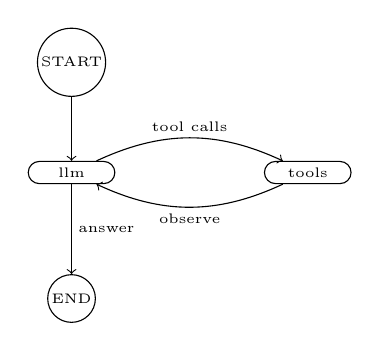
\begin{tikzpicture}
\tiny
\node[draw,circle,inner sep=1pt] (s) at (0,3.2) {START};
\node[draw,rounded corners,minimum width=1.1cm] (l) at (0,1.8) {llm};
\node[draw,rounded corners,minimum width=1.1cm] (t) at (3,1.8) {tools};
\node[draw,circle,inner sep=1pt] (e) at (0,0.2) {END};
\draw[->] (s) -- (l);
\draw[->,bend left=25] (l) to node[above] {tool calls} (t);
\draw[->,bend left=25] (t) to node[below] {observe} (l);
\draw[->] (l) -- node[right] {answer} (e);
\end{tikzpicture}
\end{center}
\tiny{The ReAct loop: the llm node and the tools node alternate until there are no tool calls.}
\end{minipage}%
}
\end{frame}

%%%%%%%%%%%%%%%%%%%%%%%%%%%%%%%%%%%%%%%%%%%%%%%%%%%%%%%%%%%
\begin{frame}[fragile]\frametitle{Setup}
      \begin{itemize}
        \item Default model: a small one on your own computer, so no API key and no per-token charge.
        \item In LM Studio, download \texttt{gemma-2-2b-it} (the Q4\_K\_M file, about 1.7 GB) and start the local server (Developer tab).
        \item One file, \texttt{llm\_config.py}, holds the model name for every example.
      \end{itemize}
\begin{lstlisting}[language=Python, basicstyle=\tiny]
pip install langgraph langchain-openai geopy requests

python llm_config.py      # prints the model ids the server offers
# put that id in MODEL_NAME, or:  LLM_MODEL=<id>   (PowerShell: $env:LLM_MODEL = "<id>")
# cloud back ends only: GROQ_API_KEY or GEMINI_API_KEY in the environment, never in code
\end{lstlisting}
\end{frame}

%%%%%%%%%%%%%%%%%%%%%%%%%%%%%%%%%%%%%%%%%%%%%%%%%%%%%%%%%%%
\begin{frame}[fragile]\frametitle{Define the State}
      \begin{itemize}
        \item The state is the \textbf{context object} that flows through every node: a Pydantic class.
        \item \texttt{add\_messages} is a \textbf{reducer}: it appends new messages and merges by message ID.
        \item The counter shows that state can hold more than messages.
        \item Shortcut: the prebuilt \texttt{MessagesState} already carries \texttt{messages}.
      \end{itemize}
\begin{lstlisting}[language=Python, basicstyle=\tiny]
from typing import Annotated
from langchain_core.messages import AnyMessage
from langgraph.graph.message import add_messages
from pydantic import BaseModel, Field

class AgentState(BaseModel):
    """The context object that flows through every node."""
    messages: Annotated[list[AnyMessage], add_messages] = Field(default_factory=list)
    number_of_steps: int = 0
\end{lstlisting}
\end{frame}

%%%%%%%%%%%%%%%%%%%%%%%%%%%%%%%%%%%%%%%%%%%%%%%%%%%%%%%%%%%
\begin{frame}[fragile]\frametitle{Define the Tool}
\begin{lstlisting}[language=Python, basicstyle=\tiny]
# geocode() and fetch_hourly() are small helpers: see react_agent.py
import json
from langchain_core.tools import tool
from pydantic import BaseModel, Field

class SearchInput(BaseModel):
    location: str = Field(description="The city, e.g., San Francisco")
    date: str = Field(description="The forecasting date, yyyy-mm-dd")

@tool("get_weather_forecast", args_schema=SearchInput)
def get_weather_forecast(location: str, date: str) -> str:
    """Retrieves the weather using the Open-Meteo API.
    Takes a city and a date (yyyy-mm-dd), returns JSON with min/max/mean."""
    coords = geocode(location)              # geopy Nominatim
    if coords is None:
        return json.dumps({"error": "Location not found"})
    hourly = fetch_hourly(*coords, date)    # requests.get(open-meteo)
    ...
    return json.dumps({"min_c": min(t), "max_c": max(t), "mean_c": avg})

tools = [get_weather_forecast]
\end{lstlisting}
\end{frame}

%%%%%%%%%%%%%%%%%%%%%%%%%%%%%%%%%%%%%%%%%%%%%%%%%%%%%%%%%%%
\begin{frame}[fragile]\frametitle{Choose the Model and Bind the Tool}
      \begin{itemize}
        \item \texttt{get\_llm()} reads the one shared config, so no example hard-codes a model name.
        \item \texttt{bind\_tools} sends the tool schema (name, description, argument types) with every request.
        \item A model that supports tools replies with \texttt{tool\_calls} instead of text. A small model may answer in plain text instead: always test this step first.
      \end{itemize}
\begin{lstlisting}[language=Python, basicstyle=\tiny]
from llm_config import get_llm      # MODEL_NAME lives in llm_config.py

llm = get_llm()                     # default: small model in LM Studio
model = llm.bind_tools(tools)

res = model.invoke("What is the weather in Berlin on 2026-10-15?")
print(res.tool_calls)
# [{'name': 'get_weather_forecast', 'args': {...}, 'id': '...'}]
# empty list: the model answered in text, so it did not use the tool
\end{lstlisting}
\end{frame}

%%%%%%%%%%%%%%%%%%%%%%%%%%%%%%%%%%%%%%%%%%%%%%%%%%%%%%%%%%%
\begin{frame}[fragile]\frametitle{The Tool Node}
      \begin{itemize}
        \item Run every tool call in the last AI message and wrap each result in a \texttt{ToolMessage}.
        \item \texttt{tool\_call\_id} links the result back to the request.
        \item The prebuilt \texttt{ToolNode} does exactly this.
      \end{itemize}
\begin{lstlisting}[language=Python, basicstyle=\tiny]
from langchain_core.messages import ToolMessage

tools_by_name = {t.name: t for t in tools}

def call_tool(state: AgentState):
    outputs = []
    for tool_call in state.messages[-1].tool_calls:
        result = tools_by_name[tool_call["name"]].invoke(tool_call["args"])
        outputs.append(ToolMessage(content=result,
                                   name=tool_call["name"],
                                   tool_call_id=tool_call["id"]))
    return {"messages": outputs}
\end{lstlisting}
\end{frame}

%%%%%%%%%%%%%%%%%%%%%%%%%%%%%%%%%%%%%%%%%%%%%%%%%%%%%%%%%%%
\begin{frame}[fragile]\frametitle{The Model Node and the Routing Edge}
      \begin{itemize}
        \item Each node reads the state (\texttt{state.messages}) and returns only what changed.
        \item The router ends the run when there is no tool call or when the step limit is hit.
      \end{itemize}
\begin{lstlisting}[language=Python, basicstyle=\tiny]
def call_model(state: AgentState):
    response = model.invoke(state.messages)
    return {"messages": [response],
            "number_of_steps": state.number_of_steps + 1}

def should_continue(state: AgentState):
    if state.number_of_steps >= MAX_STEPS:
        return "end"                       # cycle limit
    if not state.messages[-1].tool_calls:
        return "end"                       # final answer reached
    return "continue"
\end{lstlisting}
\end{frame}

%%%%%%%%%%%%%%%%%%%%%%%%%%%%%%%%%%%%%%%%%%%%%%%%%%%%%%%%%%%
\begin{frame}[fragile]\frametitle{Assemble and Visualise}
\begin{lstlisting}[language=Python, basicstyle=\tiny]
from langgraph.graph import StateGraph, START, END

workflow = StateGraph(AgentState)
workflow.add_node("llm", call_model)
workflow.add_node("tools", call_tool)
workflow.add_edge(START, "llm")                 # first node to run
workflow.add_conditional_edges(
    "llm", should_continue,
    {"continue": "tools", "end": END})          # path map
workflow.add_edge("tools", "llm")               # loop back

graph = workflow.compile()

from IPython.display import Image, display
display(Image(graph.get_graph().draw_mermaid_png()))
\end{lstlisting}
\end{frame}

%%%%%%%%%%%%%%%%%%%%%%%%%%%%%%%%%%%%%%%%%%%%%%%%%%%%%%%%%%%
\begin{frame}[fragile]\frametitle{Run the Agent and Stream the Steps}
      \begin{itemize}
        \item \texttt{stream\_mode="values"} yields the full state after every node, so each Think, Act and Observe step is visible.
      \end{itemize}
\begin{lstlisting}[language=Python, basicstyle=\tiny]
from datetime import datetime

inputs = {"messages": [("user",
          f"What is the weather in Berlin on {datetime.today().date()}?")],
          "number_of_steps": 0}

for state in graph.stream(inputs, stream_mode="values"):
    state["messages"][-1].pretty_print()

# Human Message   -> the question
# Ai Message      -> tool call: get_weather_forecast(Berlin, date)
# Tool Message    -> {"min_c": ..., "max_c": ..., "mean_c": ...}
# Ai Message      -> natural-language answer
\end{lstlisting}
\end{frame}

%%%%%%%%%%%%%%%%%%%%%%%%%%%%%%%%%%%%%%%%%%%%%%%%%%%%%%%%%%%
\begin{frame}[fragile]\frametitle{A Real ReAct Trace}
      \begin{itemize}
        \item Each streamed state adds one message to the context object; read it top to bottom.
        \item Two LLM calls and one tool call: \texttt{number\_of\_steps} ends at 2.
      \end{itemize}
\begin{lstlisting}[basicstyle=\tiny\ttfamily]
Human Message : What is the weather in Berlin on 2026-10-15?

Ai Message    : Tool Calls: get_weather_forecast
                  location: Berlin   date: 2026-10-15

Tool Message  : {"location": "Berlin", "date": "2026-10-15",
                 "min_c": 7.3, "max_c": 16.1, "mean_c": 11.4}

Ai Message    : Forecast for Berlin on 15 Oct 2026: minimum 7.3 C,
                maximum 16.1 C, mean 11.4 C. A mild day.
\end{lstlisting}
\end{frame}

%%%%%%%%%%%%%%%%%%%%%%%%%%%%%%%%%%%%%%%%%%%%%%%%%%%%%%%%%%
\begin{frame}[fragile]\frametitle{Continuing the Conversation}
      \begin{itemize}
        \item The final state already holds the whole history, so a follow-up just appends a message.
        \item The agent can re-use earlier results, call the tool again, or compare cities.
        \item For memory that survives restarts, compile with a checkpointer and pass a \texttt{thread\_id}.
      \end{itemize}
\begin{lstlisting}[language=Python, basicstyle=\tiny]
state["messages"].append(("user", "Would it be warmer in Munich?"))

for state in graph.stream(state, stream_mode="values"):
    state["messages"][-1].pretty_print()
\end{lstlisting}
\end{frame}

%%%%%%%%%%%%%%%%%%%%%%%%%%%%%%%%%%%%%%%%%%%%%%%%%%%%%%%%%%%
\begin{frame}[fragile]\frametitle{One Config, Any Model}
      \begin{itemize}
        \item Only the model line is provider-specific; state, nodes and edges stay the same.
        \item Change \texttt{MODEL\_NAME} in \texttt{llm\_config.py}, or set an environment variable, and every example follows.
      \end{itemize}
\begin{lstlisting}[language=Python, basicstyle=\tiny]
# llm_config.py (shortened)
PROVIDER   = os.getenv("LLM_PROVIDER", "lmstudio")   # lmstudio | ollama | groq | gemini
MODEL_NAME = os.getenv("LLM_MODEL") or DEFAULT_MODELS[PROVIDER]
#   lmstudio -> "gemma-2-2b-it"   (small, local, free)
#   groq     -> "openai/gpt-oss-20b"   (needs GROQ_API_KEY)

def get_llm(provider=None, temperature=None, model=None): ...

graph = build_graph(get_llm())                  # the model comes from the config
# LLM_PROVIDER=groq python react_agent.py       # same graph, another back end
\end{lstlisting}
\end{frame}

%%%%%%%%%%%%%%%%%%%%%%%%%%%%%%%%%%%%%%%%%%%%%%%%%%%%%%%%%%%
\begin{frame}[fragile]\frametitle{Prebuilt ToolNode and tools\_condition}
      \begin{itemize}
        \item The hand-written \texttt{call\_tool} and \texttt{should\_continue} are so common that LangGraph ships them.
        \item \texttt{ToolNode} runs the tool calls; \texttt{tools\_condition} routes to \texttt{tools} or END.
      \end{itemize}
\begin{lstlisting}[language=Python, basicstyle=\tiny]
from langgraph.graph import START
from langgraph.prebuilt import ToolNode, tools_condition

workflow = StateGraph(AgentState)
workflow.add_node("llm", call_model)
workflow.add_node("tools", ToolNode(tools))
workflow.add_edge(START, "llm")
workflow.add_conditional_edges("llm", tools_condition)  # tools or END
workflow.add_edge("tools", "llm")
graph = workflow.compile()
\end{lstlisting}
\end{frame}

%%%%%%%%%%%%%%%%%%%%%%%%%%%%%%%%%%%%%%%%%%%%%%%%%%%%%%%%%%%
\begin{frame}[fragile]\frametitle{One-Line Agent with create\_agent}
      \begin{itemize}
        \item \texttt{create\_agent} (LangChain 1.x, built on LangGraph) builds the whole loop; it replaces \texttt{create\_react\_agent}.
        \item By hand you saw what it does: a model node, a tool node and a router over a shared state.
      \end{itemize}
\begin{lstlisting}[language=Python, basicstyle=\tiny]
from langchain.agents import create_agent

agent = create_agent(
    model=get_llm(),
    tools=[get_weather_forecast],
    system_prompt="You are a concise weather assistant.",
)
result = agent.invoke(
    {"messages": [("user", "Weather in Berlin on 2026-10-15?")]})
print(result["messages"][-1].content)
\end{lstlisting}
\end{frame}

%%%%%%%%%%%%%%%%%%%%%%%%%%%%%%%%%%%%%%%%%%%%%%%%%%%%%%%%%%%
\begin{frame}[fragile]\frametitle{Guardrails for Tools and Steps}
      \begin{itemize}
        \item \textbf{Tools never raise into the graph}: return an error string so the model can explain or retry.
        \item \textbf{Step limit}: the counter in the state stops runaway Think, Act loops.
        \item \textbf{Validated state}: a wrong type fails at the node boundary, not three steps later.
      \end{itemize}
\begin{lstlisting}[language=Python, basicstyle=\tiny]
try:
    coords = geocode(location)
    ...
except Exception as exc:               # network, rate limit, bad date
    return json.dumps({"error": str(exc)})

def should_continue(state: AgentState):
    if state.number_of_steps >= MAX_STEPS:   # e.g. 6
        return "end"
    ...
\end{lstlisting}
\end{frame}

%%%%%%%%%%%%%%%%%%%%%%%%%%%%%%%%%%%%%%%%%%%%%%%%%%%%%%%%%%%
\begin{frame}[fragile]\frametitle{Extending the ReAct Agent}
      \begin{itemize}
        \item \textbf{More tools}: search, calculator, database; the model picks which to call.
        \item \textbf{Structured output node}: force the final answer into a Pydantic schema.
        \item \textbf{Reflection node}: critique the draft answer before returning it.
        \item \textbf{Memory}: add a checkpointer so threads resume across sessions.
        \item \textbf{Human approval}: pause before risky tools with \texttt{interrupt}.
        \item \textbf{Guardrails}: step limits, tool timeouts, retries on transient errors.
      \end{itemize}
\end{frame}

%%%%%%%%%%%%%%%%%%%%%%%%%%%%%%%%%%%%%%%%%%%%%%%%%%%%%%%%%%
\begin{frame}[fragile]\frametitle{Frugal AI: Same Graph, Smaller Model}
      \begin{itemize}
        \item The graph did not change when the model went from a cloud API to a file on your laptop. Only the model line did.
        \item What you gain: no per-token charge, no key, the data stays on the machine, and it works offline.
        \item What you check: does the small model call the tool, follow the format and stay in the step limit? Test it on your task before you trust it.
        \item Known limits of this particular model: \texttt{gemma-2-2b-it} has no system role in LM Studio's Gemma preset, so system text is folded into the first user message (\texttt{fold\_system\_prompt} in the config), and neither model card mentions tool calling.
        \item A fixed workflow with a small model is the frugal default; a free-roaming agent needs a stronger model.
      \end{itemize}
\end{frame}

%%%%%%%%%%%%%%%%%%%%%%%%%%%%%%%%%%%%%%%%%%%%%%%%%%%%%%%%%%
\begin{frame}[fragile]\frametitle{Where to Go Next: FrugalAI}
      \begin{itemize}
        \item \textbf{FrugalAI repository}: measured benchmarks and recipes for small models on old laptops and Raspberry Pi, with a small harness to measure your own device (tokens per second, memory).
        \item \textbf{Awesome list}: a curated list of frugal AI efforts by platform (old laptop, Raspberry Pi, phone, microcontroller, browser). Entries must be free to use, use a downloadable model, charge no per-token fee, and say what they were run on.
        \item \textbf{Contribute}: run something frugal? Add it to the list, or add one measurement from your own device.
        \item Students and educators are welcome to join.
      \end{itemize}
\end{frame}

%%%%%%%%%%%%%%%%%%%%%%%%%%%%%%%%%%%%%%%%%%%%%%%%%%%%%%%%%%
\begin{frame}[fragile]\frametitle{Takeaways}
      \begin{itemize}
        \item \textbf{State is the context object}: one Pydantic model flows through every node.
        \item \textbf{Nodes are plain functions}: read the state, return only what changed.
        \item \textbf{Edges decide}: one conditional edge turns a chain into a Think, Act, Observe loop.
        \item \textbf{The model is swappable}: a small local model, Groq or Gemini, same graph, one config.
        \item \textbf{Build it once, then use the prebuilt}: \texttt{ToolNode} or \texttt{create\_agent}.
      \end{itemize}
\end{frame}

%%%%%%%%%%%%%%%%%%%%%%%%%%%%%%%%%%%%%%%%%%%%%%%%%%%%%%%%%%%
\begin{frame}[fragile]\frametitle{Quick Check: The ReAct Loop}
\begin{block}{Think About It}
In the hand-written ReAct graph, what makes the loop stop and return an answer?
\begin{enumerate}
  \item[A.] The \texttt{tools} node returns END after one call
  \item[B.] The router finds no tool calls in the last AI message (or the step limit is hit)
  \item[C.] The LLM must output the word FINISH
  \item[D.] The graph always stops after two LLM calls
\end{enumerate}
\end{block}
\end{frame}

%%%%%%%%%%%%%%%%%%%%%%%%%%%%%%%%%%%%%%%%%%%%%%%%%%%%%%%%%%%
\begin{frame}[fragile]\frametitle{Quick Check: The ReAct Loop}
\begin{block}{Answer}
\textbf{Correct: B.} \texttt{should\_continue} ends the run when the model replies without tool calls, or when \texttt{number\_of\_steps} reaches the limit. Option A is wrong because \texttt{tools} always loops back to \texttt{llm}; options C and D describe rules that do not exist in this graph.
\end{block}
\end{frame}
